\onlyinsubfile{\setcounter{section}{5}}
\section{Extensions}\notinsubfile{\label{sec:exts}}

\par In this section, I describe the data and accompanying statistical model used to understand the role of \textit{financial literacy} in the current story of an empirical relationship between trust and returns.

\par Following the argument that trust is at the heart of financial agreements, the extent to which investors trust the financial institutions they make contracts with should be the sense in which trust effects returns. To test this, I redo the analysis from the main text using an aggregate measure of trust in financial institutions. 

\subsection{Financial literacy and returns}

\par Financial literacy can be an important factor when trying to understand the persistent component of returns. The literature on measuring financial literacy using survey data has agreed on three questions (the ``Big Three'') to measure financial literacy for respondents, and the HRS 2020 wave adopts the folllowing variation of these questions as a part of its survey:

\begin{enumerate}
    \item \textbf{Interest} \\
    Suppose you had \$100 in a savings account and the interest rate was 2\% per year. After 5 years, how much do you think you would have in the account if you left the money to grow? \\
    \textit{(a) Less than \$102 \quad (b) Exactly \$102 \quad (c) More than \$102}
    
    \item \textbf{Inflation} \\
    Imagine that the interest rate on your savings account was 1\% per year and inflation was 2\% per year. After 1 year, how much would you be able to buy with the money in this account? \\
    \textit{(a) More than today \quad (b) Exactly the same as today \quad (c) Less than today}
    
    \item \textbf{Risk Diversification} \\
    Please tell us whether this statement is true or false: ``Buying a single company's stock usually provides a safer return than a stock mutual fund.'' \\
    \textit{(a) True \quad (b) False}
  \end{enumerate}\footnote{\say{DK} (Don't Know) and \say{RF} (Refused) are possible non-responses for each of the questions.}

\subsubsection{Descriptive statistics}

\par Again, the persistent component of returns suggests that there is substantial variation in returns across individuals on average. Uncovering what drives these differences can be of particular interest to other literature aimed at modeling household behavior and decision problems.

\par To begin in this direction, consider in the summary for the proportion of the sample that answered each of the questions correctly in table ~\ref{tab:finlit_summary}.

\inputtable{../../Code/Descriptive/Tables/finlit_summary.tex}
\label{tab:finlit_summary}
\FloatBarrier

\par The \say{Literacy score} refers to a score between 0 and 3 showing how many of the three questions each respondent got correctly. As see from the table ~\ref{tab:finlit_freq}, almost half of the individuals answered all three correctly.

\inputtable{../../Code/Regressions/FinLit/Tables/finlit_freq.tex}
\label{tab:finlit_freq}
\FloatBarrier

\par Table ~\ref{tab:finlit_score_demographics_panels} is a breakdown of the sample performance on the financial literacy score by groupings relevant to the control variables of the empirical analysis (gender, education, age, and race).

\inputtable{../../Code/Regressions/FinLit/Tables/finlit_score_demographics_panels.tex}
\label{tab:finlit_score_demographics_panels}
\FloatBarrier

\par Along with the aggregated literacy score, the inflation question has the best performance among the measures in terms of the statistical analysis. I take a look at the same breakdown but for the \say{Inflation} in table ~\ref{tab:finlit_q2_demographics_panels}. 

\inputtable{../../Code/Regressions/FinLit/Tables/finlit_q2_demographics_panels.tex}
\label{tab:finlit_q2_demographics_panels}
\FloatBarrier
 
\par Table~\ref{tab:finlit_trust_corr} shows the cross correlations between the financial literacy measures and the general measure of trust. There is little correlation between trust and any of the financial literacy variables. More worrisome is that there is little correlation amongst the financial literacy variables. If they are all measuring the same thing, there should be some correlation. 

\inputtable{../../Code/Descriptive/Tables/finlit_trust_corr.tex}
\label{tab:finlit_trust_corr}
\FloatBarrier

\subsubsection{Results}

\par Not only is the financial literacy measure a potential determinant of differences in average returns across individuals, but it also may help to explain the variation in returns to net wealth. To consider these effects, I run each of the models of interest (cross section, average, panel specifications 1,2, and 3) with either the three financial literacy questions (interest, inflation, risk diversification) or the aggregated financial literacy score. The analysis concludes that the inflation question and the financial literacy score have predictive power for returns.

\par At the cross section, both \say{Inflation} and \say{Literacy score} are positively correlated with returns to net wealth. This can be seen in table ~\ref{tab:finlit_r5_cross_section}. Notably, both coefficients reject the null hypothesis whether or not trust is included in the regression. The coefficients for gender, education, and race retain their predictive power for returns in this setting. The Wald tests are rejected for the coefficients on age bins, wealth deciles, and race categories.  

\inputtable{../../Code/Regressions/FinLit/Tables/finlit_r5_cross_section.tex}
\label{tab:finlit_r5_cross_section}
\FloatBarrier

\par For average returns over the period, only the inflation question is explanatory for returns and retains its predictive power when trust is included. However, unlike at the cross section, the Wald test on the linear and quadratic trust terms is rejected here for both \say{Inflation} and \say{Literacy score}. Interestingly, I fail to reject the Wald tests for the coefficients on age bins, wealth deciles, and race categories in this setting based on the large p-values found in the table ~\ref{tab:finlit_r5_average}. 

\inputtable{../../Code/Regressions/FinLit/Tables/finlit_r5_average.tex}
\label{tab:finlit_r5_average}
\FloatBarrier

\par The results for the third panel regression specification ~\ref{tab:finlit_r5_panel3} are the most interesting. In the second stage of this final panel specification \textit{without} financial literacy, trust lacks significance regarding the explanatory power of variation in trust for variation in the estimated fixed effects. This was reflected in the large p-values for the tests on the individual coefficients, as well as for the joint Wald test.

\inputtable{../../Code/Regressions/FinLit/Tables/finlit_r5_panel3.tex}
\label{tab:finlit_r5_panel3}
\FloatBarrier

\par When the financial literacy variables are included in the second stage (``Big Three'' or financial literacy score), not only are those coefficients signficant, but the individual trust coefficients are now significant as well. However, the story is not all good -- the signs on the estimated coefficients for the linear trust term are negative (so the maximal economic performance does not make sense in this setting).

\subsection{Trust in financial institutions}

\par To focus specifically on the domain of trust most directly related to financial transactions, similar to \cite{Rosen2025} I construct composite measures of trust in financial institutions, aggregating responses related to trust in banks, mutual funds, and financial advisors. This targeted measure of trust is more theoretically aligned with the mechanisms through which interpersonal trust may influence realized investment returns. I present results using two aggregation strategies: (i) the simple average of the three trust scores, and (ii) the PCA analysis including those three variables and the general trust measure.

\subsubsection{Composite trust score}

\par Table ~\ref{tab:fin_trust_summary} shows average trust levels for each of the indidivual trust components used to create the \say{Trust in Fin. Institutions} variable. The sample seems more trusting of banks than financial advisors or mutual funds, which pushes up the average trust level among the three. 

\inputtable{../../Code/Regressions/Trust/FinInst/fin_trust_summary.tex}
\label{tab:fin_trust_summary}
\FloatBarrier

\par Table~\ref{tab:fin_trust_components_corr} reports pairwise correlations among general trust and the three financial-institution trust components (banks, financial advisors, mutual funds). This helps benchmark how closely the general trust measure co-moves with the institution-specific trust variables used in the extension.

\inputtable{../../Code/Regressions/Trust/FinInst/fin_trust_components_corr.tex}
\label{tab:fin_trust_components_corr}
\FloatBarrier

\par The results for this section can be summarized as follows. For the 2022 cross-section and for the average over the period, trust in financial institutions lacks explanatory power for returns to net wealth. This is reflected by the tests on the individual coefficients as well as the joint Wald test.

\par The panel regression results are slightly more favorable. For the baseline regression, table ~\ref{tab:fin_trust_avg_panel1} shows that the joint Wald test for the linear and quadratic trust term is rejected. The joint tests for age bins, wealth deciles, and race categories behaves similarly.

\inputtable{../../Code/Regressions/Trust/FinInst/fin_trust_avg_panel1.tex}
\label{tab:fin_trust_avg_panel1}
\FloatBarrier

\par I turn attention to the empirical relationship between trust in financial institutions and returns when controlling for risk exposure in table ~\ref{tab:fin_trust_avg_panel2}. The joint Wald test on the trust coefficients is rejected here as well; however, the coefficient on the linear trust term is negative. This suggests that the critical value for trust in financial institutions here does not maximize returns to net wealth.

\inputtable{../../Code/Regressions/Trust/FinInst/fin_trust_avg_panel2.tex}
\label{tab:fin_trust_avg_panel2}
\FloatBarrier

\par Lastly, results for the final panel specification on trust in financial institutions allowing for individual fixed effects can be seen in table ~\ref{tab:fin_trust_avg_panel3}. Interestingly, trust in financial institutions has strong predictive power for the individual fixed effect. In fact, the relationship appears to be hump-shaped: those with higher estimated fixed effects have moderate trust levels. 

\inputtable{../../Code/Regressions/Trust/FinInst/fin_trust_avg_panel3.tex}
\label{tab:fin_trust_avg_panel3}
\FloatBarrier

\par To assess whether the hump-shaped pattern implied by table~\ref{tab:fin_trust_avg_panel3} is visible in the data, figure~\ref{fig:fe_vs_trust_fininst_avg} plots the estimated person fixed effect against trust in financial institutions. The scatter does not show a clear inverted-U shape, suggesting caution in interpreting the quadratic fit as strong visual evidence of a hump-shaped relationship.

\begin{figure}[H]
\centering
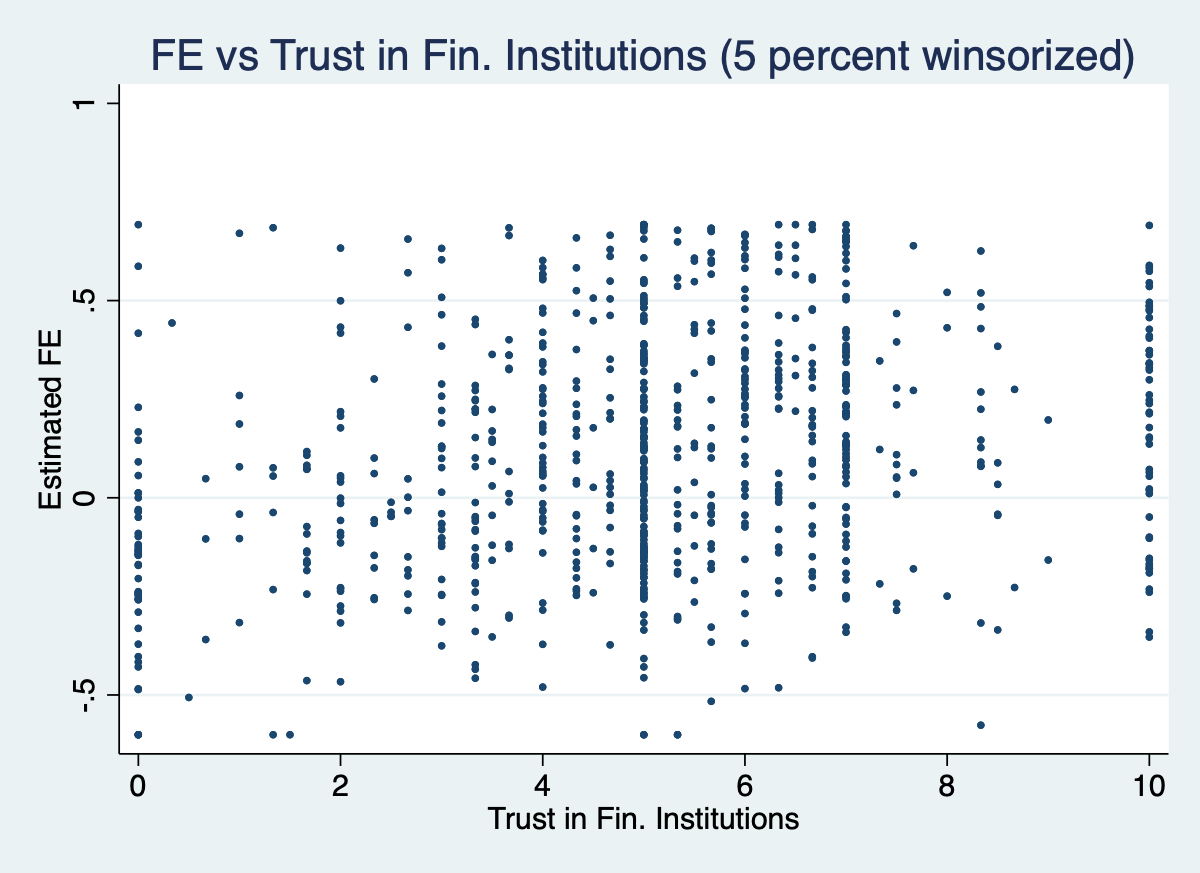
\includegraphics[width=0.8\textwidth]{../../Code/Regressions/Trust/FinInst/Figures/fe_vs_trust_fininst_avg.png}
\caption{Estimated fixed effects and trust in financial institutions}
\label{fig:fe_vs_trust_fininst_avg}
\end{figure}
\FloatBarrier


\subsubsection{Principal component analysis}

\par Principal component analysis (PCA) is a dimensionality reduction technique that transforms a set of correlated variables into a smaller number of uncorrelated components, each capturing a portion of the original variance. In the context of survey-based econometric analysis, PCA helps synthesize information from related variables—in this case, trust in financial advisors, mutual funds, and banks—into a single latent index. Including general trust alongside these financial trust variables in the PCA allows us to examine whether broader interpersonal trust co-moves with institutional trust and to what extent it contributes to the underlying factor structure.

\par Figure~\ref{fig:fin_trust_scree} displays the scree plot from the PCA analysis. The first component accounts for a significant share of the total variance, with a sharp drop in explained variance after the first eigenvalue. This suggests a one-factor structure may be appropriate, capturing a dominant dimension of trust in financial institutions. The relatively flat tail beyond the first component supports the decision to focus on the first principal component for constructing a composite measure.

\begin{figure}[H]
\centering
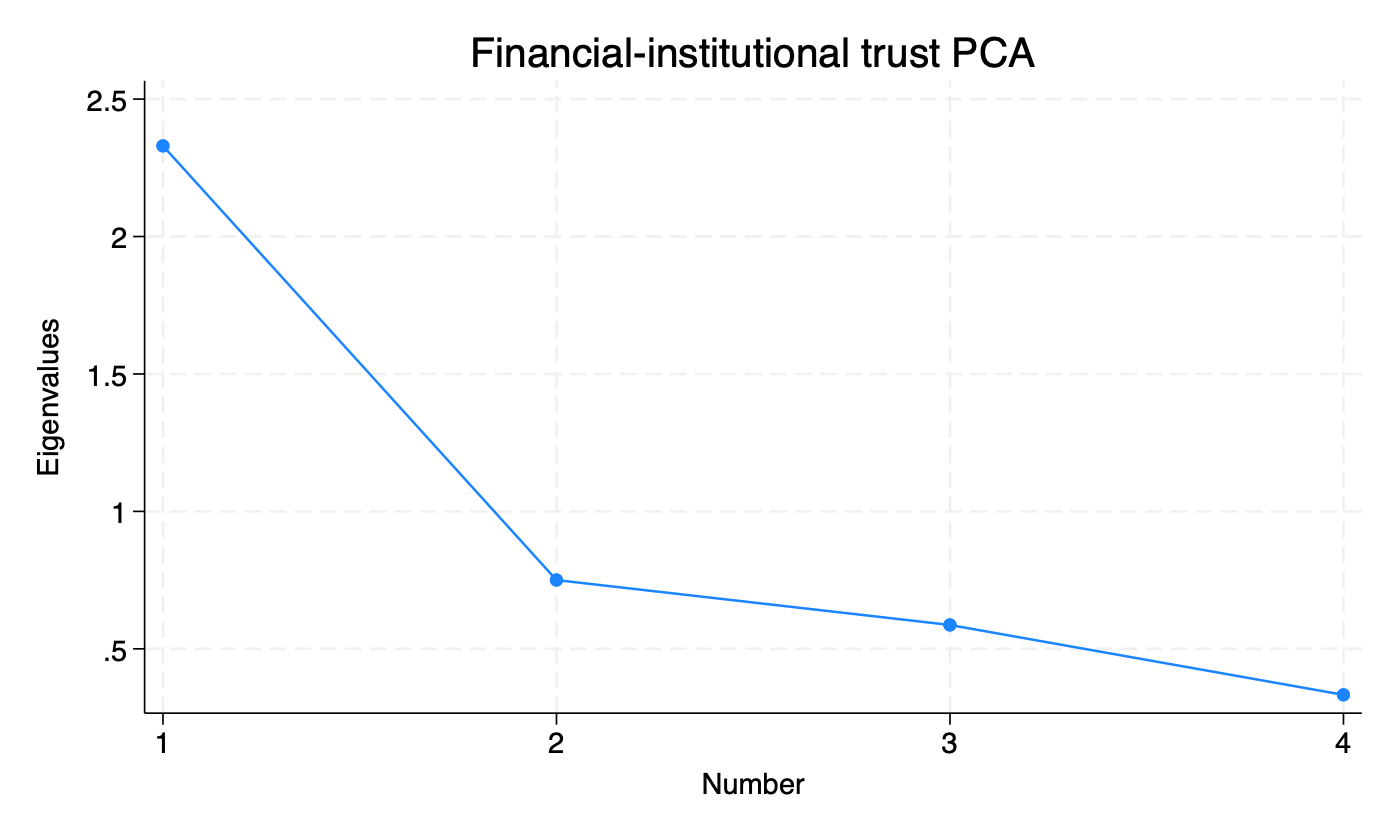
\includegraphics[width=0.8\textwidth]{../../Code/Regressions/Trust/FinInst/Figures/fin_trust_scree.png}
\caption{Financial-institutional trust PCA: scree plot}
\label{fig:fin_trust_scree}
\end{figure}
\FloatBarrier

\par Table~\ref{tab:fin_trust_loadings} presents the loadings for each trust variable on the first two components. Loadings represent the contribution of each original variable to the new principal components. In Component 1, all four trust variables load positively and similarly, indicating they move together and reflect a common latent factor—likely overall financial trust. Component 2, in contrast, differentiates general trust from the institutional trust variables, with a notably higher loading for general trust. This implies that while general trust is correlated, it may capture a broader dimension of trust beyond financial institutions.

\inputtable{../../Code/Regressions/Trust/FinInst/fin_trust_loadings.tex}
\label{tab:fin_trust_loadings}
\FloatBarrier

\par For the first component, the average-return results in table~\ref{tab:fin_trust_pc1_wgen_avg} are only modestly supportive. In the quadratic specification, the trust-squared term is negative and statistically significant, while the linear trust term is small and not statistically different from zero. The joint Wald test on the trust terms is rejected which suggests some nonlinearity, but not a strong hump-shaped pattern.

\inputtable{../../Code/Regressions/Trust/FinInst/fin_trust_pc1_wgen_avg.tex}
\label{tab:fin_trust_pc1_wgen_avg}
\FloatBarrier

\par The FE second-stage results for the first component in table~\ref{tab:fin_trust_pc1_wgen_panel3} are stronger. The linear trust coefficient is positive and significant, the quadratic term is negative and significant, and the joint Wald test is strongly rejected. This is consistent with a hump-shaped relationship, where moderate levels of financial-institutional trust are associated with higher estimated fixed effects.

\inputtable{../../Code/Regressions/Trust/FinInst/fin_trust_pc1_wgen_panel3.tex}
\label{tab:fin_trust_pc1_wgen_panel3}
\FloatBarrier

\par The regression results when using the second component differ from the first component. In table~\ref{tab:fin_trust_pc2_wgen_avg}, the linear trust term is positive and statistically significant, while the quadratic term is not significant. Although the joint Wald test is rejected, the fitted pattern is closer to a positive linear association than to a hump shape, so there is no clear interior trust level that maximizes returns.

\inputtable{../../Code/Regressions/Trust/FinInst/fin_trust_pc2_wgen_avg.tex}
\label{tab:fin_trust_pc2_wgen_avg}
\FloatBarrier

\par A similar pattern appears in the pooled panel specification in table~\ref{tab:fin_trust_pc2_wgen_panel1}. The linear trust coefficient is positive and significant, the trust-squared coefficient is not significant, and the joint trust test is rejected. Again, this points to a mostly increasing relationship over the support of the data rather than a hump-shaped one.

\inputtable{../../Code/Regressions/Trust/FinInst/fin_trust_pc2_wgen_panel1.tex}
\label{tab:fin_trust_pc2_wgen_panel1}
\FloatBarrier

\par Finally, table~\ref{tab:fin_trust_pc2_wgen_panel3} shows that in the FE second stage for the second component, both trust coefficients are negative and statistically significant, and the joint Wald test is strongly rejected (p-value 0.00). With a negative linear and negative quadratic term, this specification implies a decreasing relationship over the relevant range, so it does not imply an interior trust-maximizing point for returns.

\inputtable{../../Code/Regressions/Trust/FinInst/fin_trust_pc2_wgen_panel3.tex}
\label{tab:fin_trust_pc2_wgen_panel3}
\FloatBarrier

% \subsection{Regional and hometown trust}

% \par The literature on trust discusses the role of heterogeneity in community factors (income and race) in determining trust. The HRS RAND product which is publicly available does not have information on geographic location beyond census region. 

% \subsubsection{Desctiptive statistics}

% \par There is information in the survey about what region the respondent lives in for each wave. This along with the assumption of constant trust allows us to create a measure of regional trust. How the sample count changes by region can be seen in the table . 

% \inputtable{../../Code/Descriptive/Tables/region_group_counts_by_year.tex}
% \FloatBarrier

% \par The mean trust levels by region can be seen in the table .

% \inputtable{../../Code/Descriptive/Tables/trust_mean_by_censreg_2020.tex}
% \FloatBarrier

% \par There was also a question in 2020 asking individuals \say{how large is the population of the city, village, or town where you currently live}. The trust literature discusses how trust may vary in different communities (small, close-knit towns versus large cities). Counts by population size (6 bins) and by population in 3 bins (small town, small/medium city, large metro) are in the tables . 

% \inputtable{../../Code/Descriptive/Tables/bin_counts_population_2020.tex}
% \FloatBarrier

% \inputtable{../../Code/Descriptive/Tables/bin_counts_population3_2020.tex}
% \FloatBarrier

% \par Mean trust by population size are given in the table . 

% \inputtable{../../Code/Descriptive/Tables/trust_mean_by_population3_2020.tex}
% \FloatBarrier

% \subsubsection{Results}


% \subsection{Instrumental variables}

% \par My first attempt at identification of causal effects of trust on returns relied on literature in this direction. Specifically, inherited trust has been used as an instrument for trust before. Though I dont have a measure of inherited trust, I include some variables about the respondents' parents that is available in 2020 as an alternative. The correlations between those variables and general trust is in the figure .

% \inputtable{../../Code/Descriptive/Tables/iv_trust_corr.tex}
% \FloatBarrier
